% ======================================================
% Configuration Manual – N-of-1 ADHD + Bipolar Disorder
% Practicum Part 2 – MSc Artificial Intelligence for Business
% National College of Ireland – Rodrigo Marques Teixeira
% ✅ This template targets **pdfLaTeX** (Overleaf default) and avoids engine‑specific packages.
% ======================================================

\documentclass[12pt,a4paper]{article}

% ---------- Packages (pdfLaTeX‑safe) ----------
\usepackage[utf8]{inputenc}
\usepackage[T1]{fontenc}
\usepackage{lmodern}
\usepackage{microtype}
\usepackage{geometry}
\usepackage{graphicx}
\usepackage{booktabs}
\usepackage{longtable}
\usepackage{float}
\usepackage{caption}
\usepackage{hyperref}
\usepackage{amsmath, amssymb}
\usepackage{xcolor}

% ---------- Layout ----------
\geometry{margin=2.5cm}
\setlength{\parskip}{0.6em}
\setlength{\parindent}{0pt}
\hypersetup{
  colorlinks=true,
  linkcolor=blue,
  urlcolor=blue,
  citecolor=blue,
  pdfauthor={Rodrigo Marques Teixeira},
  pdftitle={Configuration Manual (Full) – N-of-1 ADHD + BD}
}

% ---------- Title ----------
\title{\textbf{Configuration Manual (Full Version)}\\N-of-1 Study – ADHD + Bipolar Disorder\\\vspace{0.4cm}\large Practicum Part 2 – MSc in Artificial Intelligence for Business}
\author{\textbf{Rodrigo Marques Teixeira} \\ National College of Ireland \\ Supervisor: Dr. Agatha Mattos}
\date{October 2025}

\begin{document}
\maketitle
\tableofcontents
\newpage

% ======================================================
% 1. Introduction
% ======================================================
\section{Introduction}
This manual documents the configuration and reproducibility details for Practicum Part 2. It covers ETL, modeling, explainability, and ethical governance for the N-of-1 longitudinal study on ADHD and Bipolar Disorder.

% ======================================================
% 2. System Architecture
% ======================================================
\section{System Architecture}
\textbf{Components:} data sources (Apple Health, Amazfit GTR4, Helio Ring, EMA), ETL pipeline, modeling notebooks, and SHAP explainability. Include a simple block diagram as a figure (PNG/PDF) placed under \texttt{docs/figures/} and referenced with \verb|\includegraphics|.

\begin{figure}[H]
  \centering
  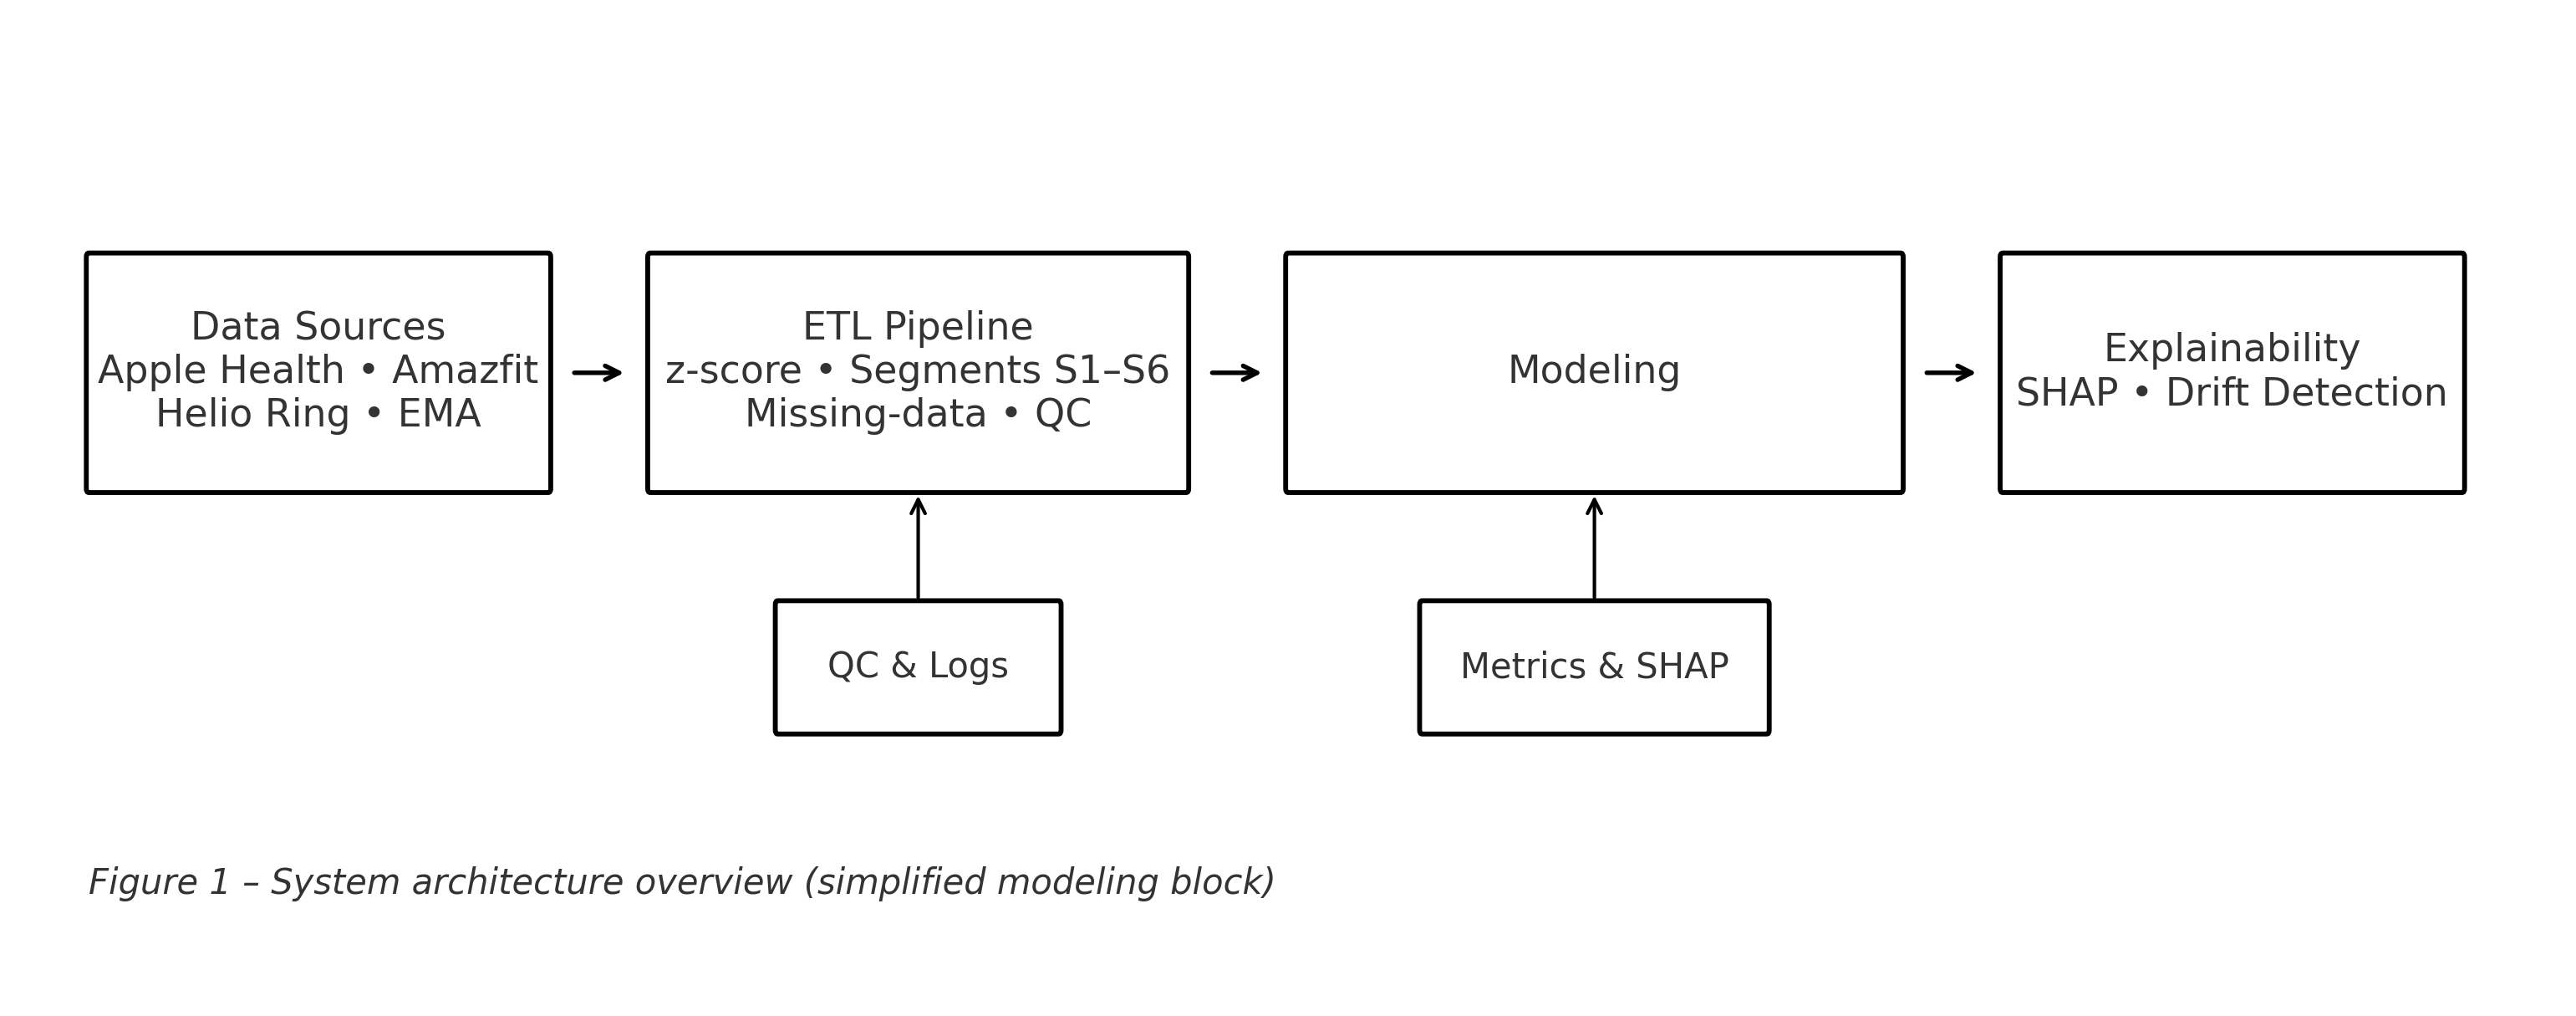
\includegraphics[width=0.9\linewidth]{docs/figures/system-architecture-paper-v3.png}
  \caption{System architecture overview with internal LSTM layers.}
  \label{fig:architecture}
\end{figure}

% ======================================================
% 3. Environment Setup
% ======================================================
\section{Environment Setup}
\subsection{Requirements}
Python 3.10+ with the dependencies listed in \texttt{requirements.txt}.

\subsection{Execution}
\begin{verbatim}
cd etl
pip install -r requirements.txt
python etl_pipeline.py
\end{verbatim}

% ======================================================
% 4. Data Management and Preprocessing
% ======================================================
\section{Data Management and Preprocessing}
Daily features are normalised per version segment $S_1,\ldots,S_6$ using z-score: $z_i = (x_i-\mu)/\sigma$. Missing values are handled via documented fallback rules. Quality checks are summarised in \texttt{etl\_qc\_summary.csv}.

\begin{figure}[H]
  \centering
  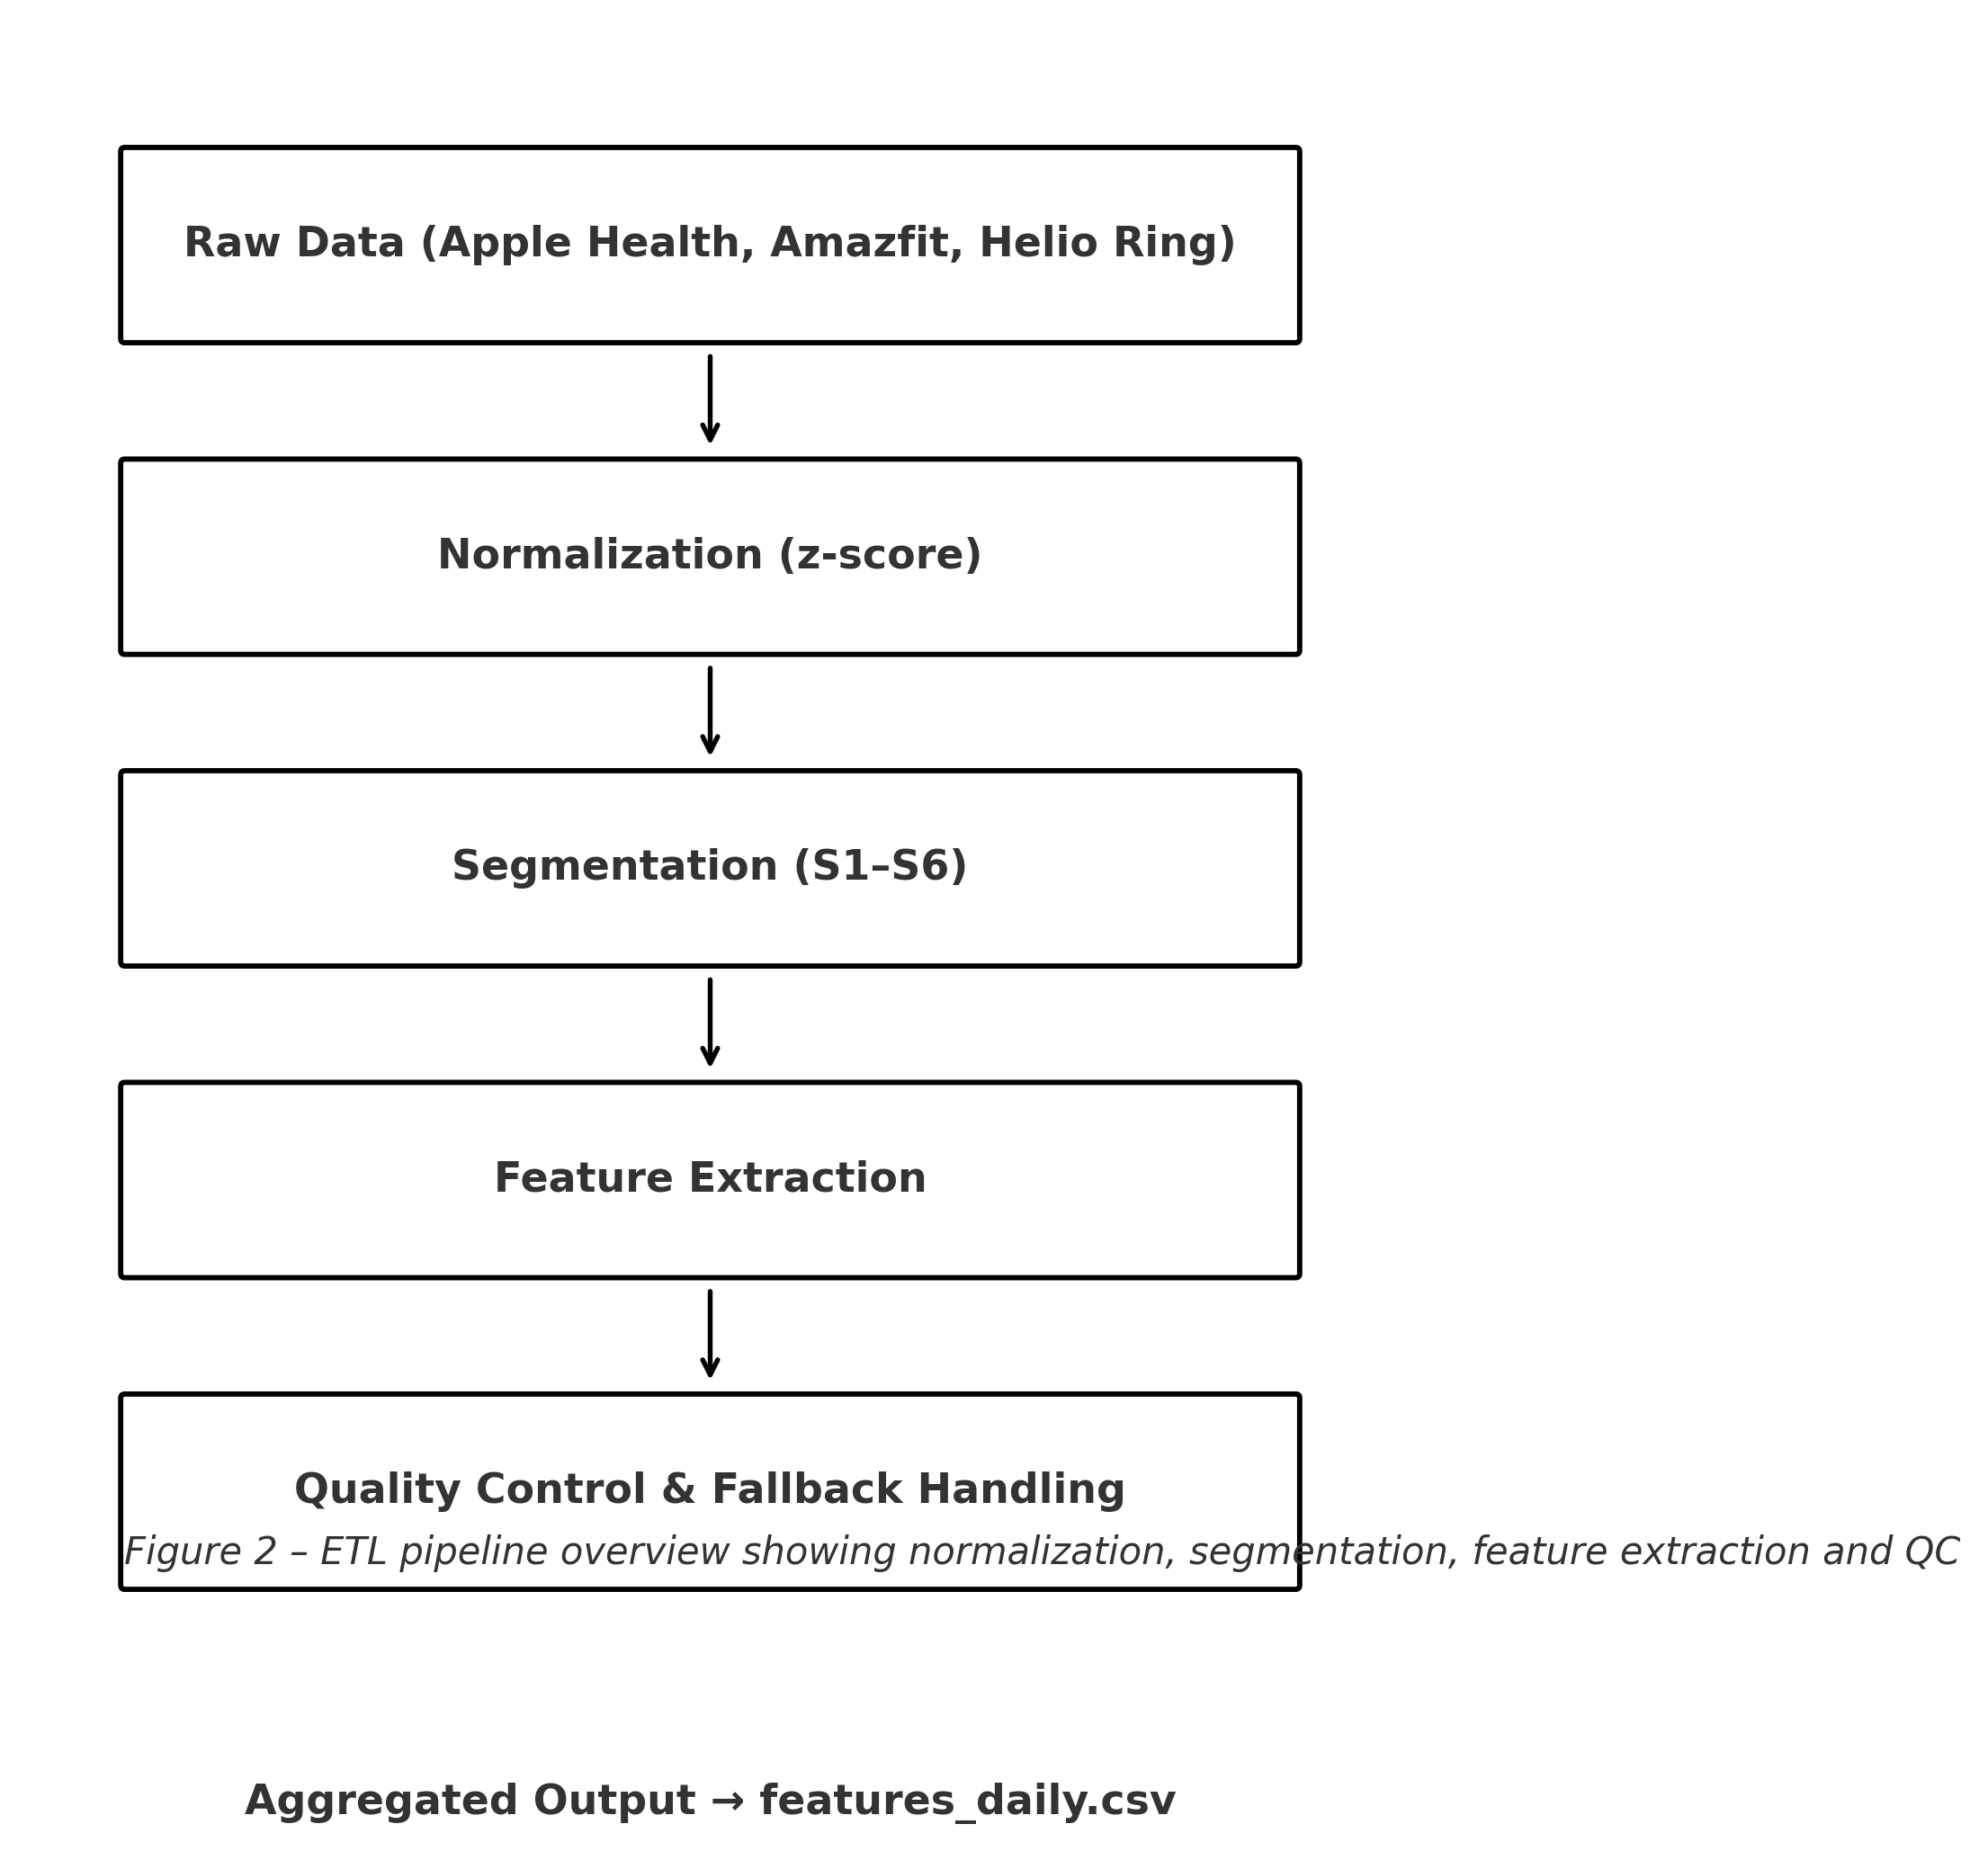
\includegraphics[width=0.75\linewidth]{docs/figures/etl-pipeline-paper.png}
  \caption{ETL pipeline overview showing normalization, segmentation, feature extraction and quality control.}
  \label{fig:etl-pipeline}
\end{figure}


% ======================================================
% 5. Modeling Framework
% ======================================================
\section{Modeling Framework}
\textbf{Notebooks:} \textit{01\_feature\_engineering.ipynb}, \textit{02\_model\_training.ipynb}, \textit{03\_shap\_analysis.ipynb}, \textit{04\_rule\_based\_baseline.ipynb}. Time-based CV uses 6 folds (4 months train / 2 months validation). Metrics: $F_1$-macro, AUROC-OvR, Balanced Accuracy, Cohen's $\kappa$, and McNemar $p$-test. The best model is exported as \texttt{best\_model.tflite}.

% ======================================================
% 6. Ethics and Governance
% ======================================================
\section{Ethics and Governance}
Phase~1: self-data. 
Phase~2: additional participants with consent and anonymisation. See documents under \texttt{docs/}.

% ======================================================
% 7. Reproducibility and Version Control
% ======================================================
\section{Reproducibility and Version Control}
The public repository contains only anonymised or synthetic samples. Version tags: \texttt{v2.0-pre-ethics}, \texttt{v2.1-ethics-approved}, \texttt{v2.2-modeling-complete}, \texttt{v2.3-final-report}.

% ======================================================
% 8. Future Work and Extensions
% ======================================================
\section{Future Work and Extensions}
Planned: S7--S9 data collection, automated drift monitoring, Helio Ring emotion via Zepp Cloud API, and clinician-backed label validation.

% ======================================================
% Appendix
% ======================================================
\appendix
\section{Appendix}
Add configuration tables, parameter grids, or pseudocode excerpts. Example inline math: $h_t = f(Wx_t + Uh_{t-1} + b)$.

\end{document}